\documentclass[12pt]{article}
\usepackage{fullpage,graphicx,psfrag,amsmath,amsfonts,verbatim}
\usepackage[small,bf]{caption}

\input defs.tex

\bibliographystyle{ieeetr}

\title{Bitcoin UTXO Lifespan Prediction}
\author{Robert Konrad \& Stephen Pinto}

\begin{document}
\maketitle

\section{Background \& Motivation}
The Bitcoin crypto currency~\cite{Na08}, born in 2009, still maintains its position as the most widely used and highly valued digital currency in existence. Every day sees thousands of transactions added to the blockchain. The blockchain is a global, agreed-upon ledger of every transaction that has ever occured and is continually extended as a single linked list. Each transaction in the blockchain, say Alice paying Bob 10 BTC, has one or more transaction outputs (TXO) which serve as sums of spendable BTC. These unspent sums are called \emph{Unspent Transaction Outputs} (UTXO). They remain UTXOs until the owner (Bob in our example) redeems them to pay someone else (at which time they are referred to as spent TXOs).

\begin{figure}
\begin{center}
\includegraphics[width=0.7\textwidth]{figures/utxo}
\end{center}
\caption{Illustrated Explanation of a UTXO. An arbitrary amount of time may pass before Bob spends his UTXO.}
\label{utxo}
\end{figure}

This project seeks to predict how long a TXO will remain unspent. More formally, given some information about the beginning transaction which created the UTXO and some information about the Bitcoin market on the day of its creation, this project predicts which of ten broad time scales the UTXO lifespan will fall into. This predictor could inform broader applications such as anomaly/fraud detection, trade volume and volatility prediction, and individual spending habit modelling. The Bitcoin industry is worth billions of dollars and growing rapidly. Possible insights into the previosly mentioned topics would be of use to any number of financial institutions involved in the future of cryptocurrencies. 



\section{Dataset \& Features}
One of the (many) blockchain explorers, Blockchain.info, has a public API exposing data about individual transactions as well as general Bitcoin market statistics. A python script queried Blockchain.info at a polite rate to gather 13146 training samples and then exported the data to a Matlab readable format. A Matlab script then curated the data into a matrix with the features listed in figure~\ref{features}.

\begin{figure}
\begin{center}
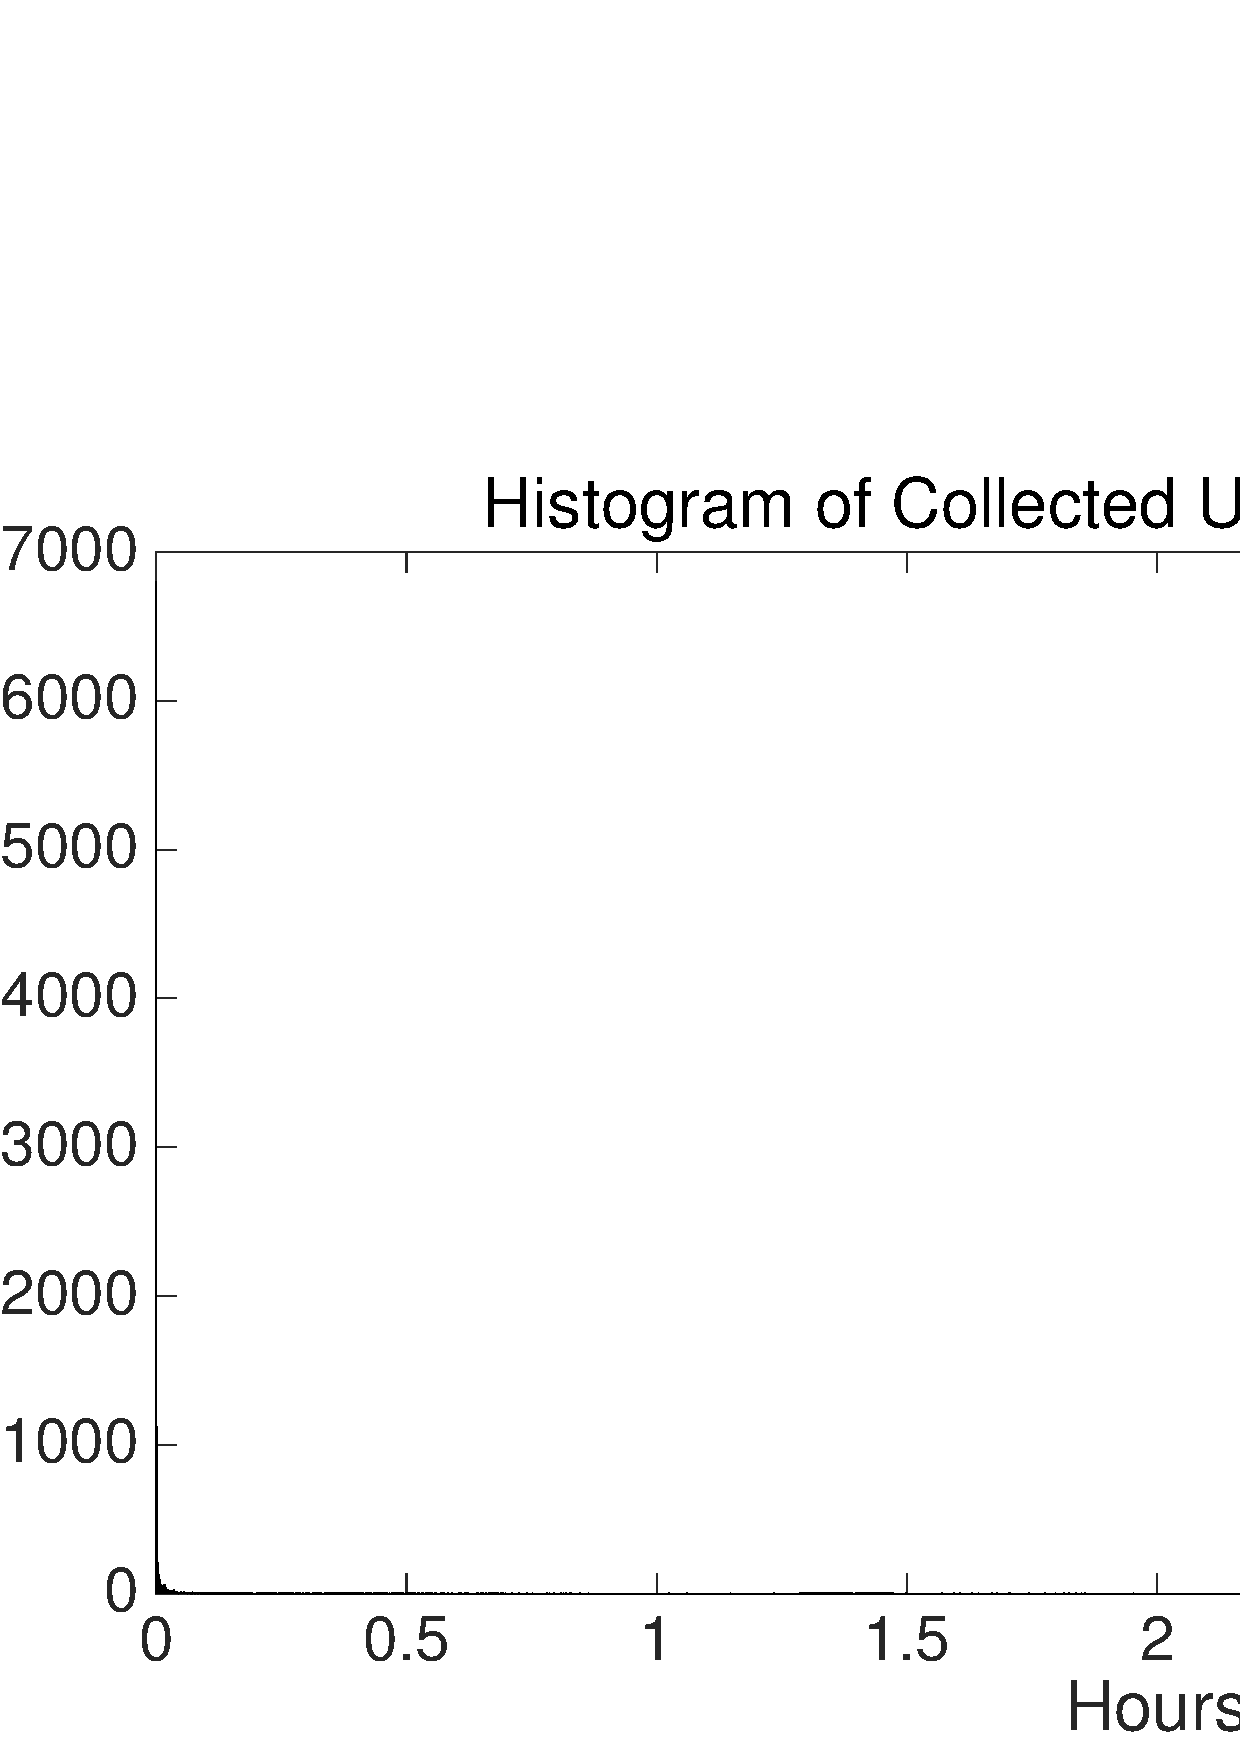
\includegraphics[width=0.9\textwidth]{figures/hist.png}
\end{center}
\caption{The histogram of collected UTXO lifespans with two regions magnified.}
\label{hist}
\end{figure}

The feature set consists of (1) information pertaining to the individual beginning transactions, and (2) information about the bitcoin market statistics on the day of creation.

We dummy coded the weekday with the reference day being Sunday. This created 6 new binary features, where each feature dictates whether the transaction occurred on a particular day. Sunday, the reference day, is represented by these 6 features being 0. The UNIX time of beginning transaction corresponded to the number of hours that occurred since the Epoch time, Thursday, 1 January, 1970. The 11th feature, transaction volume on creation date, corresponds to to the total number of unique Bitcoin transactions that occurred on the day of creation. The final three features are the three 2nd order polynomial parameters that fit the last week's USD to BTC conversion rate.

\begin{figure}
\begin{center}
\includegraphics[width=0.9\textwidth]{figures/features}
\end{center}
\caption{The features used as inputs to the classifier .}
\label{features}
\end{figure}


\section{Methods}
As shown in figure~\ref{hist}, the tail of the UTXO Lifespan distribution is extremely long. As such, regression might lead to prediction errors that are large enough to remove their useful meaning. Classification into a finite set of lifespan bins (defined by ranges of time) clarifies this issue and provides more intuitive results. The trick, however, is to define useful, data-dependent time ranges. Hardcoding these based on eyeballing the distribution seemed meaningless so we chose to instead split the full domain into ten equal-probability ranges.

Two methods of doing this are either (1) entirely empirically or (2) based on a fitted distribution. The former case is simply a matter of sorting the lifespan dataset and splitting it into ten equally sized groups. The latter requires more processing. Understanding that the data should show signs of a Laplace or exponential distribution based the standard application of those distributions, the first step was to cluster the lifespan set using k-median ($\ell_1$ penalty function) clustering. From there, we fitted either a Normal, Laplace, or Exponential (whichever was most likely) distribution to each cluster using maximum likelihood estimation and then formed a global distribution as a weighted sum. 

\begin{figure}
\begin{center}
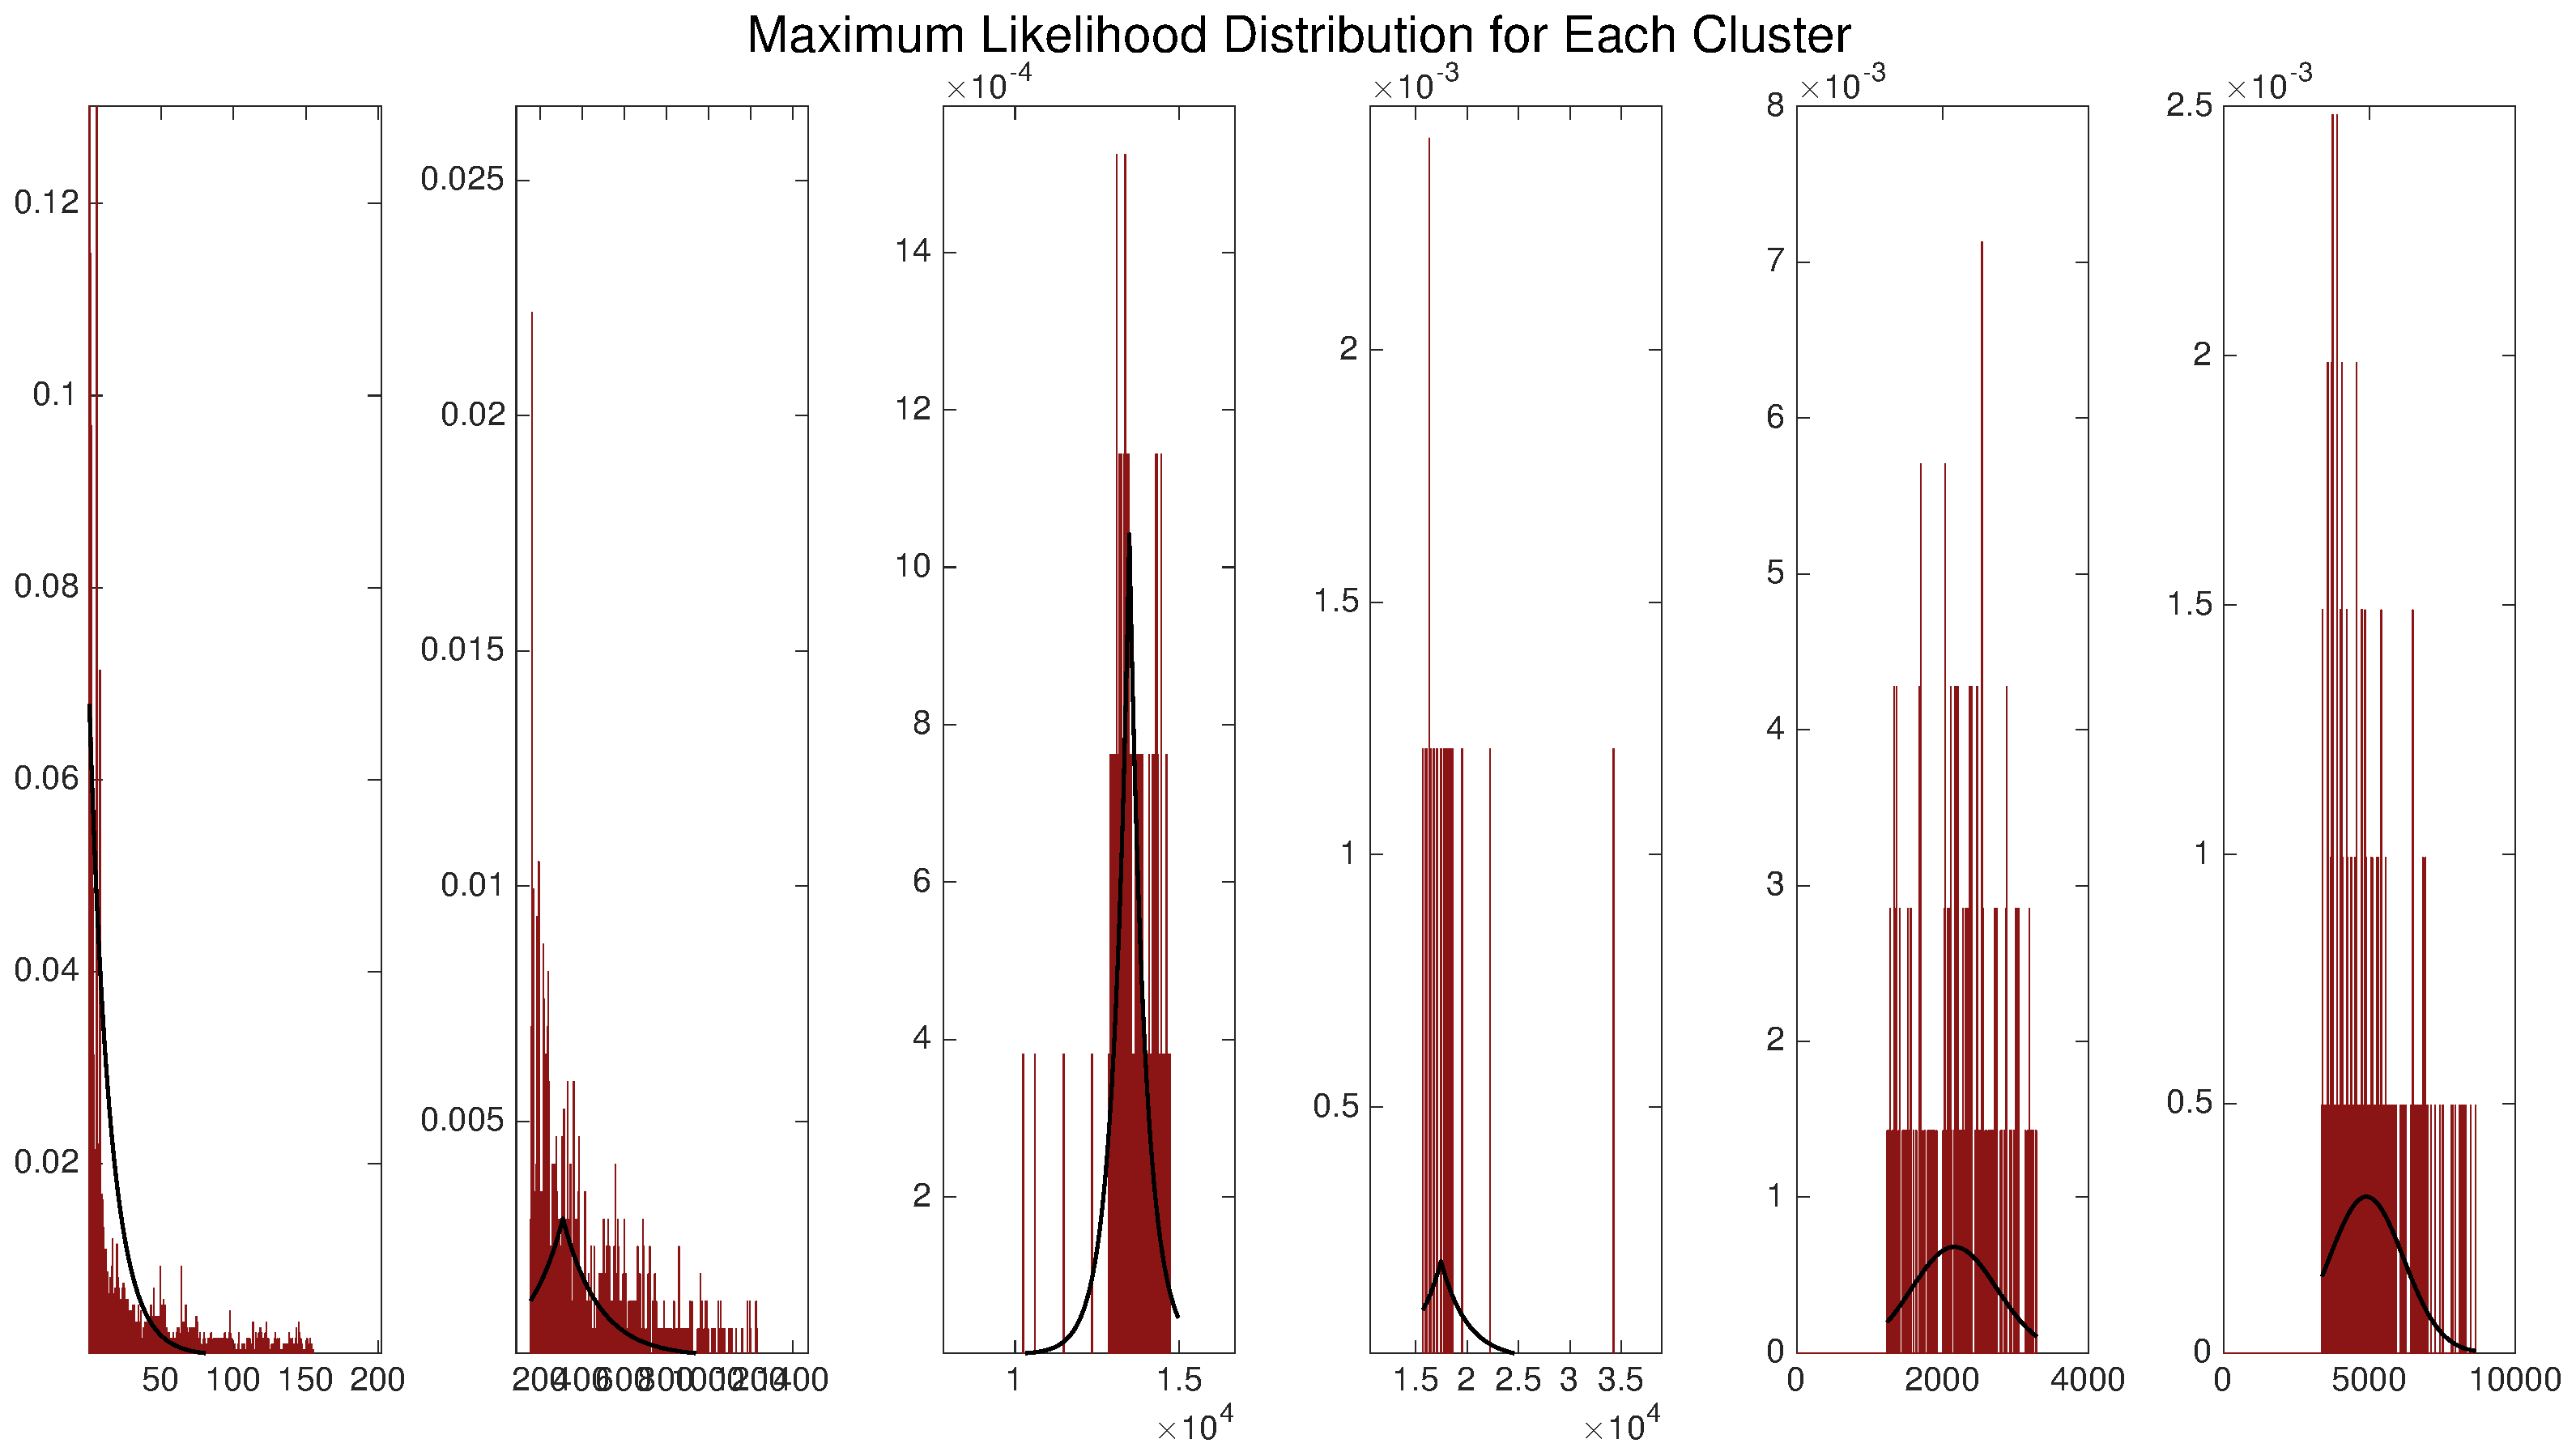
\includegraphics[width=0.9\textwidth]{figures/fits}
\end{center}
\caption{Illustrated Explanation of a UTXO. An arbitrary amount of time may pass before Bob spends his UTXO.}
\label{fits}
\end{figure}

The ten subdomains for each method are shown in tables~\ref{opt1} and~\ref{opt2} respectively.

\begin{center}
\begin{tabular}{r||c|c|c|c|c|c|c|c|c|c}
Upper Bound of Subdomain & 2 m & 10 m & 31 m & 80 m & 3 h & 7 h & 1 d & 3 d & 2 wk & $\infty$\\
\% of Dataset in Subdomain & 10 & 10 & 10 & 10 & 10 & 10 & 10 & 10 & 10 & 10
% \caption{Table of subdomain boundaries and the distribution of datapoints within subdomains for empirically calculated subdomains.}
\label{opt1}
\end{tabular}
\end{center}

\begin{center}
\begin{tabular}{r||c|c|c|c|c|c|c|c|c|c}
Upper Bound of Subdomain & 2 h & 4 h & 6.5 h & 9.5 h & 12.5 h & 17.5 h & 1 d & 1.5 d & 2 wk & $\infty$\\
\% of Dataset in Subdomain & 44 & 8 & 7 & 5 & 2 & 2 & 3 & 3 & 16 & 10
% \caption{Table of subdomain boundaries and the distribution of datapoints within subdomains for subdomains from a fitted distribution.}
\label{opt2}
\end{tabular}
\end{center}


\section{Results}

\begin{figure}
\begin{center}
\includegraphics[width=0.9\textwidth]{figures/paramSearch}
\end{center}
\caption{Classifier performance vs $\gamma$ and $C$. One region of the broader heatmap is magnified for higher granularity.}
\label{paramSearch}
\end{figure}

\begin{figure}
\begin{center}
\includegraphics[width=0.9\textwidth]{figures/error}
\end{center}
\caption{Test and training error vs size of data set using 5-fold cross validation.}
\label{error}
\end{figure}

\bibliography{btc-learning}

\end{document}